
\documentclass[12pt,letterpaper]{article}

\usepackage[utf8]{inputenc}
\usepackage[spanish]{babel}
\usepackage{times}
\usepackage[left=3cm,top=2.5cm,bottom=2.5cm,right=2.5cm]{geometry}
\usepackage{graphicx}


\begin{document}
\begin{figure}[h!]
\centering
\paragraph{UNIVERSIDAD POLITECNICA DE LA ZONA METROPOLITANA DE GUADALAJARA}
\

\

\includegraphics[scale=0.8]{Upzmg.png} 
\end{figure}
\begin{center}
\textbf{\LARGE Practica 8}\\
\end{center}
\begin{center}
\textbf{\LARGE EV\_ 3\_ 1\_ Diagrama\_ eléctrico\_ de la interfaz de potencia.}
\end{center}


\large{Integrantes:}\\
\large{Guzman Vazquez Jaime Alan.\\
Perez de Alba Santiago Eduardo.\\
Romero Jauregui Osvaldo.\\
Cabrera Gutierrez Raul.\\
Gutierrez Olivares Rogelio.\\
Rodriguez Lopez Francisco Javier.\\

Fecha: 10 de Noviembre del 2019.\\

Curso: Sep-Dic 2019.\\

Carrera: Ingenieria en Mecaronica.\\

Docente: Moran Garabito Carlos Enrique.\\}

\newpage


\section{Introducción:}

Este documento hablara a cerca de la practica que se realizo anteriormente, la practica consiste en generar  con un voltaje de entrada pequeño un incremento de voltaje en la salida del circuito mediante capacitores y push button, esta parte sera mejor explicada en el apartado de desarrollo en donde se hablara a cerca de todas las condicionantes de este tipo de circuito, así como los riesgos que podría traer puesto a su gran inestabilidad y sus beneficios grandes como el incremento grande del voltaje.\\
\\De este reporte resaltaremos dos grandes partes que son el apartado de resultados y el apartado de desarrollo en donde el apartado de desarrollo explicara el como se armo el circuito, las variables que intervinieron en el mismo, como podemos controlar el cambio mismo del incremento de voltaje y su velocidad de descarga así como los factores que lo intervienen.\\
\\
El apartado resultados mostrara las evidencias o variables que fueron salieron del mismo circuito para que el apartado desarrollo tenga coherencia y ser muestren lo que el circuito físico nos demostró, esta sera básicamente la dinámica que se manejara en este reporte de practica para demostrar el circuito realizado. \\

Ademas de los puntos ya mencionados también se hablara acerca de las diferentes aplicaciones de este circuito debido a su peculiaridad y forma de operar así como de sus características y como puede ser implementado en el ámbito profesional o empresarial y como se liga este circuito con el que se estudiara próximamente con la practica numero 9 que esta trata  de disminuir el voltaje en el circuito.


\section{Objetivo:}
Conocer el arreglo, para el paso de corriente alterna a directa, por medio de capacitores, y diodos.\\ 

\section{Materiales:}
\begin{itemize}
\item Capacitores electroliticos (100uF a 63v, 220uF a 50Vv, 10uF a 50V).
\item Diac.
\item Potenciometro de 100k.
\item Puente de diodos (RS206L).
\item Resistencias (2.2k y 100k).
\item Transformador (127vca-16vca).
\item Triac (TYN1225N).
\end{itemize}
\newpage
\section{Procedimiento:}
Para el mejor entendimiento de esta practica, se establece, las formas y arreglos que se les puede dar a la transformación de corriente alterna a continua, siendo está la forma en la que mas comúnmente se hace, que es a través de capacitores, y diodos, para la rectificación, y el almacenamiento de la carga que va transmitiendo la fuente de poder a la que lo estamos alimentando en este caso, a un to,a corriente directo, para la buena implementación de esto, el transformador, se pone, como una fuente de poder, la cual transforma la energía alterna, y hace que en su traspaso, por su embobinado, se traspase, a un voltaje alterno menor, de criterio este, nos funciona, para un regulador de corriente, así pues, guiando todo el problema al transformador, y no a nuestro circuito.\\

El diagrama a realizar en esta practica, y evidencia, es en generación, eso, poder tener el control, en la , que se tenga que manejar la corriente y el voltaje alterno, y como este nos puede ser de ayuda, a la realización de una fuente mas sofisticada, y de mayor arreglo, en términos de energía alterna. El diagrama utilizado es en cuestión el siguiente:\\

\begin{center}
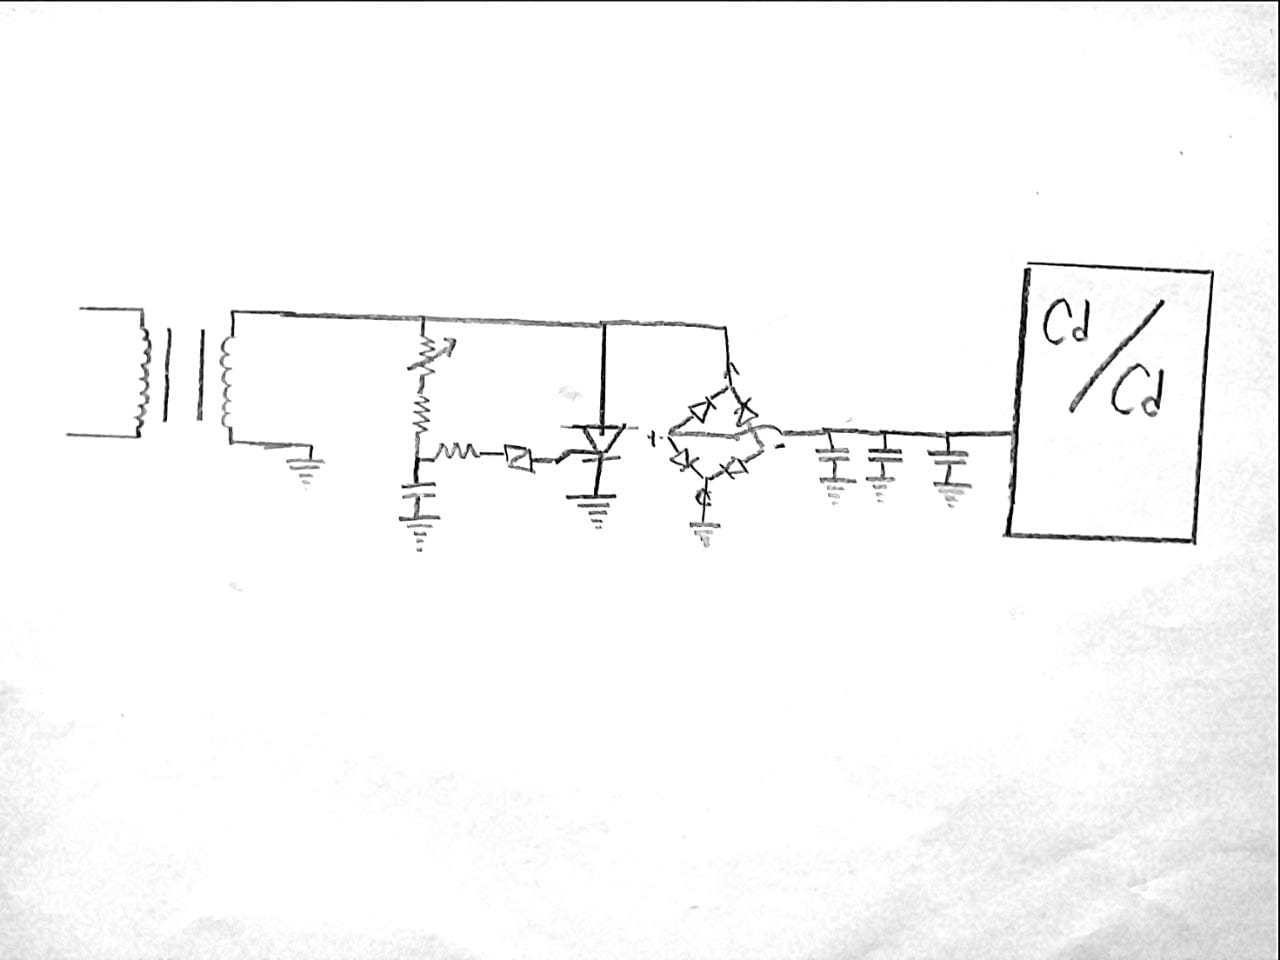
\includegraphics[width=10cm]{esquema.jpeg} 
\end{center}

Como se muestra en el esquemático, esta es el arreglo, que se tiene que tener por etapas, para la conmutación de la potencia disipada, a partir del voltaje y corriente transmitidos. Esto se tiene por etapas, siendo la etapa 1, la entrada del transformador, esto es lo que hace la conductividad posible, ya que el campo magnético que genera al ser, mayor, retrae el voltaje hasta cierto punto el cual sea manejable. La segunda etapa dirigida por el Triac, este es de suma importancia, que sea de dura potencia, ya que si no lo es, se empezara a calentar, nuestro sistema de control, que en este caso, es para regular el flujo de corriente, y que este no sea excesivo, la etapa 3, constituida, por la entrada del puente rectificador, y los capacitores, esta zona, es la que regula de mejor estancia, la salida de voltaje, potencia y corriente, que lo establece en este punto a directa, y la entrada del Boost, o convertidor de voltaje CD/CD, dobla el voltaje que tenemos a la salida, generando asi, un total de 32v en salida de corriente directa, el cual manejamos, con un Triac (MOC-502R) de menor potencia, que el puesto en primera estancia, ya que a este punto, no se necesita de una potencia grande, por que la conmutación de corriente alterna, ya a sido convertida y establecida.\\

Teniendo en claro, cada una de las etapas, a manejar, y de ello, a establecer en las pruebas físicas, nos queda establecido, un sistema de CA a CD, en control absoluto, recalcando, que en la primera estancia, se requiere de componentes, de alta potencia, ya que la corriente que se arroja, a partir de la conexión directa al enchufe, es de mayor intensidad, y los componentes, de baja potencia, no resistirían.\\

Nota: Se requiere, de un potenciometro, para la mejora de regulación, a partir de la descarga que sufran los capacitores.

\section{Resultados:}

Establecido, cada una de las etapas, a manera física, comprobadas en la protoboard, no queda un sistema de convertidor, alterna directa, apartir de la rectificación, y capacitancia, que se tenga, y como esta queda establecida, en este punto, en este caso, siendo un convertidor, de mejor y mayor control, estableciéndolo, en una interfaz de potencia, tal y como se ha estado trabajando, a lo largo de este curso, desde baja potencia, hasta potencia alta, los resultados generados, son en cuestión, la generación del brinco de corriente, hasta el doblado de la misma, controlando todo, con el mismo Triac, que se tiene a disposición misma.\\

El armado de este, genera los resultados ya mencionados, y la resolución de ellos, a partir de la generación de potencia que se tenga, y como es que se tenga esta potencia disipada. Quedando en manera física de la manera siguiente:

\begin{center}
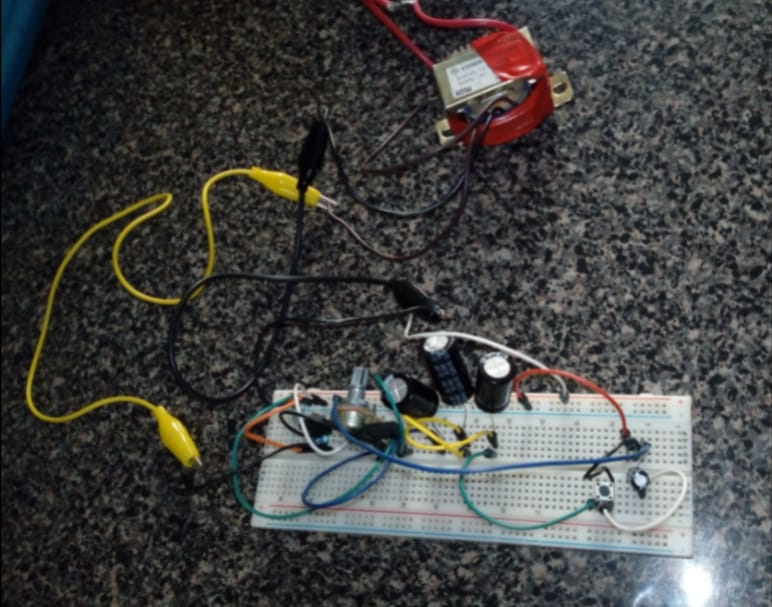
\includegraphics[width=9cm]{Fisico.jpeg} 
\end{center}

La generación y el acomodo, que se le da a nuestra protoboard, es la generación de la resultante, la cual es el lanzamiento, del voltaje de corriente directa, como se aprecia el potenciometro, en generación y control a la potencia que es disipada, en el sistema y como esta es controlada por el Triac que es conectado, en generación y siendo este conectado no de forma directa al transformador, sino, pasando por un control, de sistemas conmutados, tales, como resistencias, y un Diac, el cual nos garantiza el mejor control y sin fallas, de la rectificación que se tenga en el ánodo del Triac, así como en el gatillo.\\

Las pruebas, para tenerlo mas en cuenta, es la guia de un multimetro, para ver el voltaje que se genera a partir del paso que hace la corriente, conectando las puntas de prueba, una a la salida de los condensadores, y otra directa a tierra, ya que este punto de las tierras, se sabe que todas son comunes, y de ello, las conexiones sin riesgo, de quemar, el circuito, ni el multimetro.

\section{Conclusión:}
\begin{itemize}
\item \textbf{Jaime Guzmán:}\\
Este circuito boost es un circuito que tiene implicaciones muy útiles puesto que mediante el uso de capacitores puede hacer que el voltaje de salida sea mucho mayor al valor de entrada con capacidades dependiendo de el valor del capacitor un incremento de hasta 6 veces mas de lo se tenia de valor de entrada, lamentablemente este circuito es muy inestable por lo que podría se peligroso puesto que este podría tener cambios bruscos de voltaje o incluso poder generar cortos circuitos en el mismo, por este tipo de cuestiones este circuito no es tan seguro pero sin embargo tiene aplicaciones reales en el mundo de la electrónica ya que puede estabilizarse.\\

\item \textbf{Francisco Ródriguez:}\\
La generación, y el controlamiento de la potencia que puede ser disipada, a partir de los componentes utilizados, en un sistema de rectificación y condensación, es algo que se utiliza de manera eficiente, en sistemas mas complejos, como la prueba de ello, la practica realizada, a partir de la generación del doblador de voltaje, así como el paso, por sistemas mas comunes, como potencia de alta estancia, la cual es mas común utilizar esto, en sistemas, de proyectos mecánicos, el cual tenga que generar a partir de la gran potencia disipada, el movimiento de motores, así como de sistemas de movimiento en los cuales se necesite, un campo magnético mejor y de mayor corriente.\\
Dado el aprendizaje generado, a partir de estas practicas, y de un sistema de estudios, es lo que nos puede dar guía, a la mejor utilización de esto, para la generación de un proyecto, el cual requiera, de los conocimientos, de potencia, control de ello, y un sistema el cual nos pueda ser de eficiencia, mayor que un simple vídeo de youtube.\\
\item \textbf{Santiago Perez}\\
Durante el desarrollo de esta practica se pudo observar el funcionamiento del circuito Boost, el cual nos permitía elevar un voltaje menor y obteniendo un voltaje de salida mucho mayor, esto gracias a pulsos PWM que permiten el incremento de voltaje, el unico inconveniente encontrado con este circuito efectivo en distintas aplicaciones es que es algo inestable provocando daños al circuito adaptado, se puede lograr estabilizar mediante la implementacion de un regulador de voltaje.
\item \textbf{Osvaldo Romero}\\
En los distintos circuitos que se armaron a lo largo de las practicas, este en especifico es muy particular dado que a su configuración o función de poder aumentar nuestro voltaje, herramienta que es demasiado útil si hablamos de circuitos electrónicos de potencia
\item \textbf{Roger Gutierrez}\\
La practica nos instruye en lo útil que es un convertidor boost dentro de un circuito ya que tiene la peculiaridad de aumentar la tension de entrada teniendo una salida de mayor magnitud ya que se trata de un convertidor CD-CD esta practica aporta mucho para nuestros trabajos en lo que se necesiten tensiones mas altas que las que se tienen solucionando problemas que puedan tener próximamente en la carrera como en la vida misma.
\item \textbf{Raul Cabrera}\\
El boost es una aplicación importante en la industria, ya que las maquinas que la industria maneja necesitan altas corriente y con esta práctica a menor escala en la que se empleo el boost con la finalidad de adentrarnos un poco a lo grande que es la industria. El boost tiene muchas aplicaciones industriales porque el pulsador(boost) trabaja eficientemente ya que a partir de un voltaje fijo, otro valor de tensión mayor o menor da la salida, se puede decir que se convierte de CD a CD.
\end{itemize}
\textbf{\Large Referencias:}\\

Carlos Enrique Moran Garabito, Sistemas Electronicos de Interfaz, Curso: Sep-Dic 2019 c, Diagramas electricos de interfaz de potencia.

\end{document}